\section{Introduction}

Atomistic simulation is shifting from a case-by-case analysis tool to a predictive engine for materials discovery, molecular design and non-equilibrium process modelling.
This shift changes what is expected from an interatomic potential: it must retain density-functional-theory (DFT) accuracy, remain stable in long molecular-dynamics trajectories, transfer across chemical environments and be inexpensive enough for high-throughput use.
Machine-learning interatomic potentials (MLIPs) have made this goal plausible by replacing repeated electronic-structure calculations with near-linear-cost surrogate potential-energy surfaces~\cite{behler2007generalized,bartok2010gaussian,zhang2018deep,batzner2022nequip,batatia2022mace}.
Early and widely used MLIP families achieve this by encoding each atomic neighbourhood through invariant descriptors or scalar message-passing features, including atom-centred neural-network potentials~\cite{behler2007generalized}, Gaussian approximation potentials~\cite{bartok2010gaussian}, SchNet~\cite{schutt2017schnet}, PhysNet~\cite{unke2019physnet}, Deep Potential~\cite{zhang2018deep,wang2018deepmd} and the DPA series~\cite{zhang2022dpa,zhang2024dpa2,zhang2025dpa3}.
The recent emergence of pretrained large atomistic models (LAMs), such as M3GNet~\cite{chen2022universal}, CHGNet~\cite{deng2023chgnet}, MatterSim~\cite{yang2024mattersim}, Orb~\cite{neumann2024orb,rhodes2025orbv3}, UMA~\cite{wood2025umafamilyuniversalmodels} and DPA3~\cite{zhang2025dpa3}, shows that large DFT datasets can support transferable potentials across broad regions of chemistry and materials space.
\WH{the mace series is missing!}

The next challenge is no longer accuracy alone, but the joint optimisation of accuracy, efficiency and physical robustness.
Equivariant architectures address the accuracy side of this problem by carrying directional information as first-class features instead of compressing it immediately into invariant scalars.
NequIP~\cite{batzner2022nequip}, Allegro~\cite{musaelian2022learning}, MACE~\cite{batatia2022mace}, Equiformer-family models~\cite{liao2023equiformerv2,liao2026equiformerv3} and eSEN~\cite{fu2025esen} have demonstrated that equivariance can substantially improve data efficiency and benchmark accuracy.
However, the most expressive SO(3)-equivariant models rely on Clebsch--Gordan tensor products or dense spherical-grid operations whose cost grows rapidly with angular order, model width and neighbour count.
This cost becomes a bottleneck when the target is not a single specialised potential, but an MLIP architecture that can scale to broad training sets and serve as the backbone of future LAMs.
\WH{mention SO(2) equiv irreps product by \cite{passaro2023reducing}, eSEN is based on SO(2) convlution, and eqv3.}
\WH{perhaps explicitly say that the edge irreps are invariant. we have extended it to equivariant and equivariant irreps multiplication in SO(2) with a sparse representation of the edge irreps.
}

Efficiency and robustness impose further constraints on practical MLIP design.
Conservative-force training can be difficult to accelerate because the force loss differentiates through the energy model, so mainstream AI optimisation stacks developed for first-order LLM training do not directly apply to this second-derivative setting.
The short-range region of the potential-energy surface is also sparsely sampled in ordinary DFT datasets.
External Ziegler--Biersack--Littmark (ZBL) corrections can repair the asymptotic repulsion~\cite{ziegler1985}, but native and smooth coupling is preferable when the model is used in molecular dynamics.
These considerations motivate an architecture that treats directional expressiveness, training efficiency and short-range robustness as coupled design requirements rather than separate add-ons.

\begin{figure}[t]
    \centering
    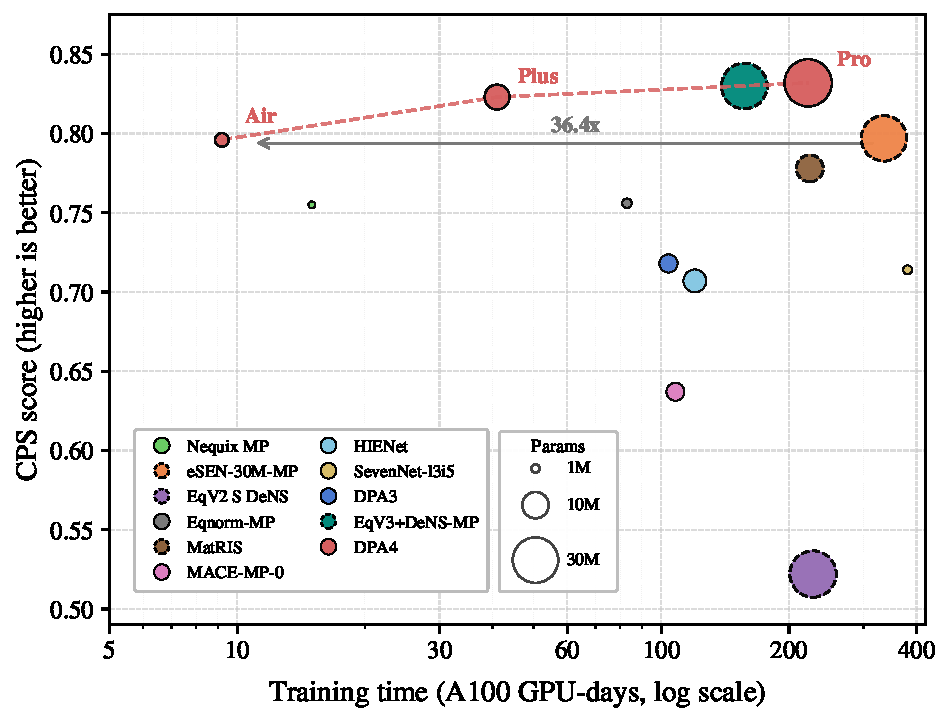
\includegraphics[width=0.6\linewidth]{fig/fig1_CPS.pdf}
    \caption{
        CPS score versus training cost for representative MLIPs.
        Marker area is proportional to the number of model parameters, and the x-axis uses a logarithmic scale of A100 GPU-days.
        Dashed marker outlines indicate models trained with additional strategies such as direct-force pre-training or DeNS.
    }
    \label{fig:cps}
\end{figure}

Here we present DPA4, an equivariant interatomic-potential architecture designed around these three requirements.
DPA4 combines local-frame equivariant message passing, compiler-friendly conservative-force training and native analytical short-range coupling in one model family.
Its main contributions are as follows.
\WH{item 1 is not our contribution. should be entirely reframed.
  novel architecture design: (0) GIE, (1) sparse edge equivariant irreps, enable edge-node equivariant product, high capacity. (2) multi-focus, lower cost higher capacity. (3) attention. (4) Lebedev SO(2) FFN.
}
\begin{enumerate}
    \item \textbf{SO(2)-equivariant local-frame architecture with attention.}
          Inspired by eSCN~\cite{passaro2023reducing}, DPA4 represents directional information in an edge-local frame, where the residual symmetry is SO(2) and equivariant updates avoid full SO(3) Clebsch--Gordan tensor products.
          Attention over invariant channels makes neighbourhood aggregation adaptive while preserving equivariance.
    \item \textbf{End-to-end \texttt{torch.compile} training.}
          DPA4 uses a shape-stable and compiler-friendly implementation of conservative force training.
          This makes the energy-to-force path compatible with \texttt{torch.compile} and provides a 2--3$\times$ wall-clock training speedup in controlled ablations.
    \item \textbf{Native ZBL Zone Bridging.}
          DPA4 incorporates the analytical ZBL repulsion inside the energy model instead of applying it as a post-hoc correction.
          A smooth Zone Bridging mechanism suppresses the direct learned short-range pair channel, preserving conservative forces while assigning the singular close-contact interaction to the analytical branch.
\end{enumerate}
DPA4 variants form a new accuracy--efficiency frontier on Matbench Discovery~\cite{riebesell2025matbench}, as summarized by the CPS-versus-training-cost comparison in Fig.~\ref{fig:cps}, and improve the molecular benchmark errors on SPICE-MACE-OFF~\cite{kovacs2023mace}.
\WH{full name of CPS}
The largest DPA4 variant reaches state-of-the-art Matbench Discovery performance, while compact variants approach the accuracy of much larger baselines with substantially fewer parameters and lower training cost.
We present DPA4 here as a single-task, per-dataset MLIP architecture; multi-task training for LAMs are natural extensions rather than assumptions of the present study.
\WH{reason why choosing Matbench Discovery and SPICE-MACE-OFF? many not be here but should be discussed in the result part: medium size (non-trivial but not too heavy, idealy for validating model architecture), strong ``out-of-domain'' genralization test.}
\WH{mention multi-task in conclusion, perspective part.}

The remainder of the paper is organized as follows.
Section~\ref{sec:results} first gives an overview of the DPA4 architecture, then reports its accuracy on Matbench Discovery and SPICE-MACE-OFF, its training and inference efficiency, its native ZBL coupling behaviour, and controlled ablations of the main architectural and systems components.
Section~\ref{sec:discussion} discusses the implications and limitations of these results.
Section~\ref{sec:methods} describes the architecture, datasets, training protocol and compiled conservative-force implementation in detail.

% =============================================================
